\chapter{Testing}
\label{Testing}
This chapter holds the overall testing results and test information about the final program. 
During implementation the program was only ever run in a single environment, \textbf{room 1}.
In this chapter the results of running the program in different environments are documented. The environments differ in shape and size as well as well as in obstacle population.

\section{Overall Approach to Testing}
As the program requires an simulator to be run in, it is not possible to test the program in any other way than to run it in an simulator and document the results. This factor makes also automatic unit testing impossible. During implementation the program was only ever tested in a single environment called \textbf{room 1}. All changes which were done to the code and problems which were documented in early chapters have been the result of the robots performance in this environment. \\[3ex]

The reason the program was never tested in different environment during implementation was since the program was not complete enough, it was assumed that before the program can be tested in multiple environments a solution for a simple environment must exist.\\
It is worth noting at this point that the project is \textbf{not} considered finished, however time restrictions do not allow for continued development.  

\section{Test environment: Room 1}
\label{room1}
Room 1 is the "original" environment in which the program was implemented. \\
It is a simple, empty, room which size is 10x10 squares, figure \ref{room1_empty} shows this environment. In order to measure the environment size the chess board pattern which makes up the floor of the simulator environment is used to measure it. \textbf{FIXME(enter size of a square in code)}\\

\begin{figure}[h]
\centering
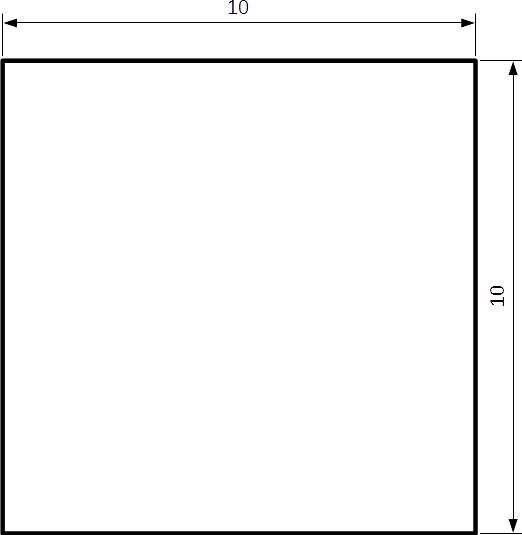
\includegraphics[width = 0.5\textwidth]{../../figures/room1_empty.png} 
\caption{Room 1 empty test environment}
\label{room1_empty}
\end{figure}

\subsection{Obstacle free test}

The results gathered in this test environment, as it is the simplest, as well as the environment in which the program was developed are by far the best in from of final result. \\

\begin{figure}[h]
\centering
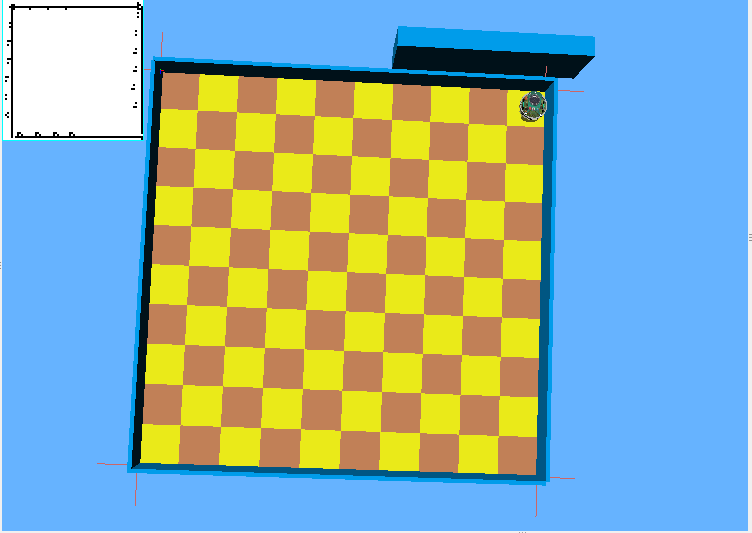
\includegraphics[width = 0.5\textwidth]{../../figures/map_results/result_room1_empty.png} 
\caption{Room 1 empty environment result}
\label{room1_empty_result}
\end{figure}

Figure \ref{room1_empty_result} shows the result of the environment after the map has been "closet". The resulting map clearly depictures the spotty nature of the U-turn mapping which is described in Chapter 3 subsection \ref{deployment_improvement} on page \pageref{deployment_improvement} . \\[3ex]

The generated map shows that the program is able to generate straight and accurate mappings of an environment as long as the robot is able to reset its odometry values at some point during the run. More info of what can happen if the odometry is not reset can be found \textbf{FIXME(enter section of page of describe accumulated odometry error)}. \\
The reason of why the program performs this well in the test environment compared to other environment is that is able to reset its odometry values by passing \textbf{corner 1}, before it moves to the uncharted \textbf{corner 2}. More information about the corner approach can be found \textbf{FIXME(link to section and page of corner approach describtion)}. \\
That the accumulated odometry error was growing constantly during program runs can be seen at the placement of the spots of the u-turn routine, these spots are marked red in figure \ref{room1_empty_marked}.

\begin{figure}[h]
\centering
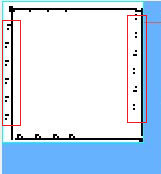
\includegraphics[width = 0.5\textwidth]{../../figures/room1_result_marked.png} 
\caption{Room 1 map result with marked odometry dislocation}
\label{room1_empty_marked}
\end{figure}

If these spots are compared to the one at bottom and top site of the generated map, it can be clearly seen that the odometry location error was crowing, and became very noticeable after the map had been generated about 50\%.\\[3ex]

However the odometry location error was reset as the robot reached \textbf{corner 1}, which X and Y coordinates were saved as the robot traversed said corner for the first time. \\
This reset the odometry values of the odometry struct and made it possible to continuously map the environment with good results. \\ 
\textbf{FIXME(enter figure and page of the figure which shows  the location error)}.\\[3ex]

However this test environment is not without shortcomings either. If the program is allowed to keep working and mapping the environment the odometry error is increasing again.\\

\begin{figure}[h]
\centering
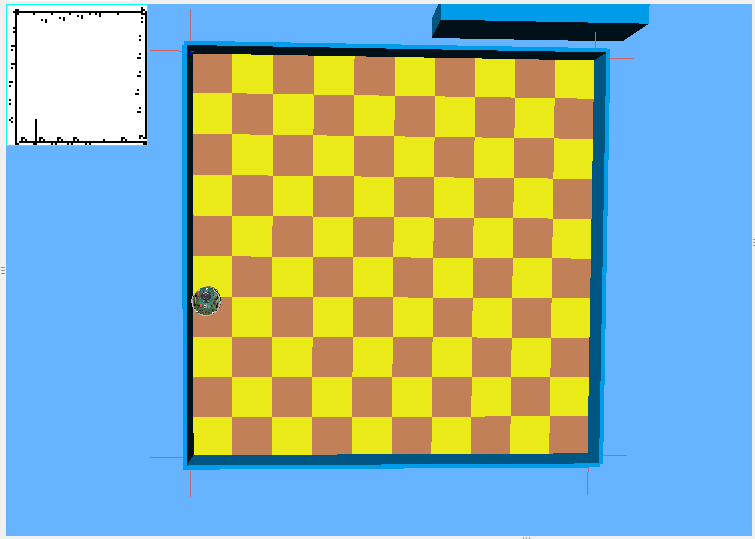
\includegraphics[width = 0.5\textwidth]{../../figures/map_results/odometry_error_and_reset.png} 
\caption{Room 1 map result with crowing odometry error}
\label{room1_empty_reset}
\end{figure}

Figure \ref{room1_empty_reset} shows the accumulated odometry error after the environment has been traversed approximately 2 times. \\
As can be seen in this figure the odometry location error keeps accumulating even though it has been reset a few times, at \textbf{corner 1} and \textbf{corner 4}. But the mapped line which can be seen on the lower left corner of the generated map indicates that the localisation error became to big so  that an area was map in the middle of the environment which clearly belongs to the left hand wall. 
This however is also an working example of the reset function which has been implemented for the corners of the environment. As the location information of the odometry struct have been reset as the corner was reached. The reset can be seen as the robot depicted in the figure already did another pass along the left hand wall up and down, after being reset in the lower left corner. \\[3ex]

This localisation error however is a rather random event, as different results from other runs suggest that the odometry error is strongly based on the random nature of the noise in the simulator. 

\begin{figure}[h]
\centering
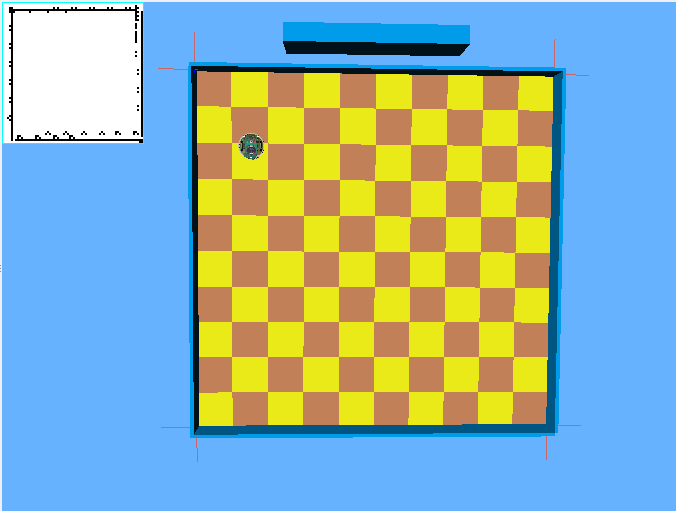
\includegraphics[width = 0.5\textwidth]{../../figures/map_results/simulator_noise_mapping.png} 
\caption{Room 1 map result with different odometry error}
\label{room1_simulator_noise}
\end{figure}

Figure \ref{room1_simulator_noise} shows the result of another test run, here the robot only had a small miss mapping issue in the upper-right corner of the map, which happened right after the map was closed. However this error was only in a small area, and was completely reset when it reached the lower-right corner of the environment. The test run depicted in this figure has progressed further than the test run shown in figure \ref{room1_empty_reset}, and it shows that the odometry localisation error did not happen again, in the same place.\\
In other test runs the odometry localisation error did not happen until the robot started traversing the environment the 3rd time, however 90\% of times before it happened during the 2nd environment traverse, this suggest that the problem lies within the random nature of the simulator, however that this random nature is within boundaries. 

\subsubsection{Conclusion for this test environment}
While the mapping performs reasonably well within this test environment not all test runs are the same. The mappings differ minimal in places every simulation run, this happens because of the random nature of the simulator. \\
While the mapping of the whole environment can be performed with reasonably similar results, the results start to differ a lot more when the robot traverses the environment a 2nd or 3rd time. The figures \ref{room1_empty_reset} and \ref{room1_simulator_noise} are the results of 2 different simulator runs which happened directly after another. Other times the 2nd simulator run returned no mapping error which was more noticeable than the common minor dis-localisation, but major errors as shown in these figures happened in later runs. The mapping error de-pictured in both documents that while the simulator random nature causes minimal map differenced every time, larger errors happen more seldom and more randomly. 

\subsection{Environment with obstacles}
\label{room1_obstacles}
This subsection shows and describes the results of another test environment. \\
This environment is the same as described in the previous sub-section however this has an obstacles added to it.

\begin{figure}[h]
\centering
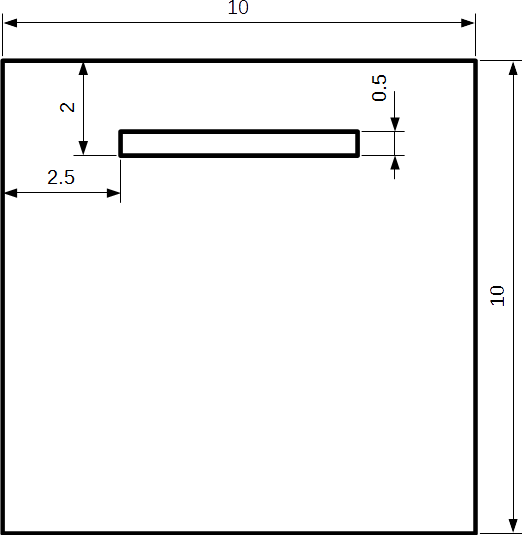
\includegraphics[width = 0.5\textwidth]{../../figures/room1_obstacle.png} 
\caption{Measurements of room 1 with obstacle added to it}
\label{room1_obstacle}
\end{figure}

Figure \ref{room1_obstacle} shows the measurements and location of the obstacles added to the environment, again all measurements are in \textit{squares}. 

\begin{figure}[h]
\centering
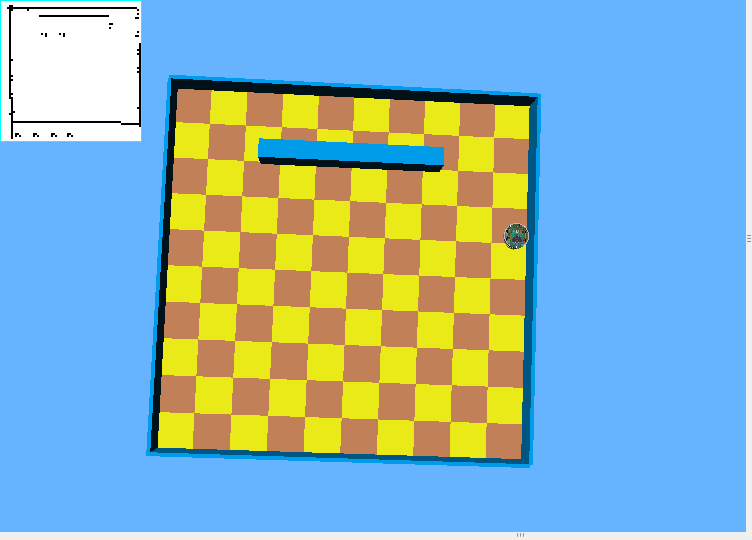
\includegraphics[width = 0.5\textwidth]{../../figures/map_results/one_obstacle_save_error.png} 
\caption{Room 1 with obstacle map result}
\label{room1_obstacle_result}
\end{figure}

Figure \ref{room1_obstacle_result} shows the result for this environment.\\
As it can clearly be seen, this figure de-pictures the major short comings of the final program. On the lower part of the generated map, it can clearly be seen where the major short coming of this solution, the odometry localisation error gets to big. \\
Unlike to the \textbf{room 1} example without any obstacle, which is described in the previous section, this result depicts what happens when the robot is not able to reach a saved reference point(already traversed and saved corners), but rather continues mapping without being reset. \\[3ex]

What has happened in this case is that the obstacle prevented the robot to traverse the whole width of the map, which altered the movement enough for the robot to reach the unsaved lower-right corner of the map before it reached an already saved reference point which would led to the localisation information being reset. \\
This can cause a couple of problems. The biggest of them is, which can be clearly seen, that the localisation error gets to large for the map to be usable. The problem in this case is that the odometry information of the lower-right corner are saved, and every time the robot passes this corner the odometry information will be updated to the saved, wrong, information.\\[3ex]

Besides this major error, it also shows the programs short comings in the mapping of obstacles which are placed in the middle of the room.  

\begin{figure}[h]
\centering
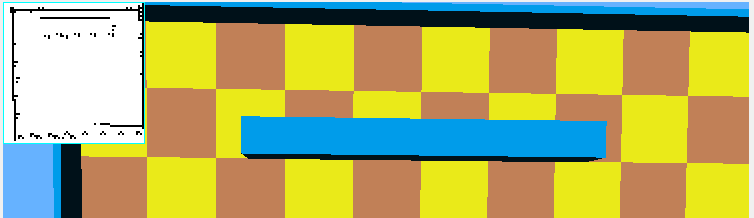
\includegraphics[width = 0.5\textwidth]{../../figures/map_results/obstacle_mapping_error.png} 
\caption{Obstacle mapping shortcomings}
\label{obstacle_mapping_error}
\end{figure}

Figure \ref{obstacle_mapping_error} shows the problem when an obstacle in the middle of the room is being mapped with the current mapping approach. \\
The upper-side of the obstacle is mapped reasonable well, however the the other sides are lacking. There are some spots on the right side of the obstacle which have been marked by during the U-Turn routine, however the lower-side of the obstacle shows the real short comings. When the mapping of the lower and the upper side of the obstacle are compared it gets clear that the main limitation with this approach is the usable mapping only happens when the robot traverse the obstacle which its side to it, so that it will be mapped. The spotty mapping points generated by the U-Turn routine are usable to outline the obstacle at best, however the specified movement pattern implemented in this project can prevent possible mapping of an obstacle should the obstacle be placed at a point which will not be passed by during the robot movements pattern. \\[3ex]

Another problem is the odometry error in an environment like this. As has already be shown the localisation error gets to big and the altered movement pattern prevents the robot from resetting its localisation values, that is not without it getting reset to something wrong when it passes a long the reference point which has been saved with the wrong odometry data in the first place, in this case the lower-right corner. \\
This however does not only cause errors for the outline of the environment but also for the obstacles, as in some simulation runs visible localisation difference on the spotty outline of an obstacle can be seen. \\[3ex]

\begin{figure}[h]
\centering
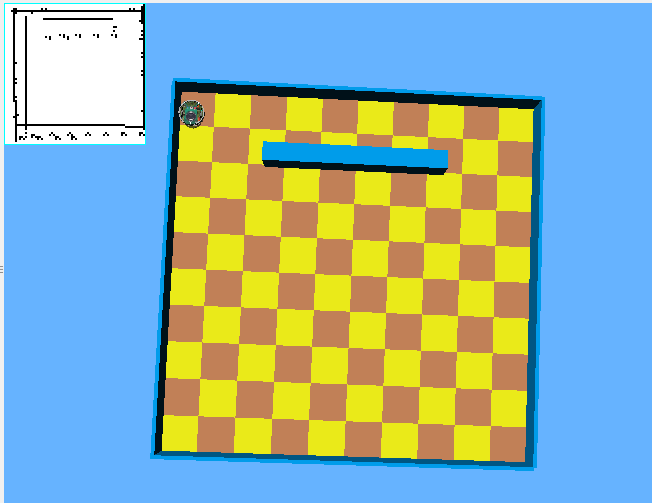
\includegraphics[width = 0.5\textwidth]{../../figures/map_results/one_obstacle_odometry_error.png} 
\caption{Accumulated odometry error}
\label{one_obstacle_odometry_error}
\end{figure}

Figure \ref{one_obstacle_odometry_error} shows the map result at a later point during the environment traverse. The figure shows how much the localisation errors accumulate  over time when the robot is not able to reset its localisation values. \\
It shows the already discussed localisation error for the lower side of the map, as well as the spotty outlining in the obstacle. However this map shows also that the localisation values have been reset in the corners which were passed before the localisation error became to big, as the spotty mappings on the lower side of the map show. While the entire lower wall of the environment is mapped at a wrong place, the localisation values have been reset in the upper right corner which causes the spotted, U-Turn based,  mappings a long the lower right hand side.\\

\begin{figure}[h]
\centering
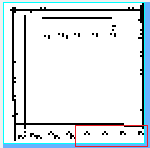
\includegraphics[width = 0.5\textwidth]{../../figures/map_results/dotted_odometry_error.png} 
\caption{Marked spots}
\label{dotted_odomery_error}
\end{figure}

In figure \ref{dotted_odomery_error} these spots have been marked. The spots to the left hand side of the marked spots have been mapped after the robot had started, since it starts in the center of the map facing to the lower end of the environment. \\
As the marked spots are approximately at the Y axes as the other markings, can be seen that the robot resets its localisation values to the correct values when it passes the upper-corner reference point. \\
However this figure also depicts what the accumulated odometry errors cause to an already scanned side. On the left hand side of the figure it can easily be seen where the robot remapped the left hand wall of the environment.\\

\subsubsection{Conclusion for this test environment}
This test environment shows the short comings of this program, the fast movement pattern can cause problems when mapping obstacles as the robot will only ever move in the same movement pattern. This however can, and in most cases will, lead to an large accumulation of localisation error.\\
It is apparent that the major problem of this program is that the odometry values need to be reset in given intervals in order to prevent an to large accumulation of errors. This is however, with the current solution, only possible when the robot manages to pass by an saved reference point before the localisation error either becomes to large, or another reference point is set with the wrong localisation information.\\[3ex]

There are a couple of ways the problems which become apparent in this test environment could have been fixed. One possibility is to have a wall following algorithm which allows for the mapping of the outline of an obstacle before falling back into another movement pattern. \\
This would prevent problem with the mapping of obstacle which has been discussed in the previous section. Another solution would be to set reference points more often, or have a way of localizing the robot besides having set reference points, possibilities for this would be GPS or long range scanners which are able to keep track of global reference points, which have been set previous to the run.\\
There are a couple of possibilities which could have been implemented in order to make this mapping better, however the problems encountered during implementation have taken to much time to fix to be even able to map a single, empty, environment to be able to implement further algorithms after test runs had been done for environment with obstacles inside them.

\section{Room 2}
Room 2 is an narrower version of \textbf{room 1}, with a size of 6x10 squares.

\begin{figure}[h]
\centering
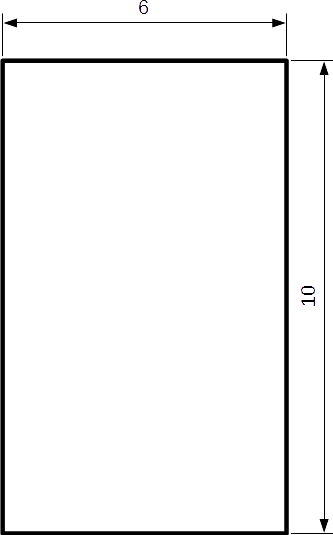
\includegraphics[width = 0.5\textwidth]{../../figures/room2_empty.png} 
\caption{Room 2 measurements}
\label{room2_empty}
\end{figure}

\subsection{Obstacle free test}
In this section the results for the obstacle free version of \textbf{room 2} will be shown and discussed. \\[3ex]

\begin{figure}[h]
\centering
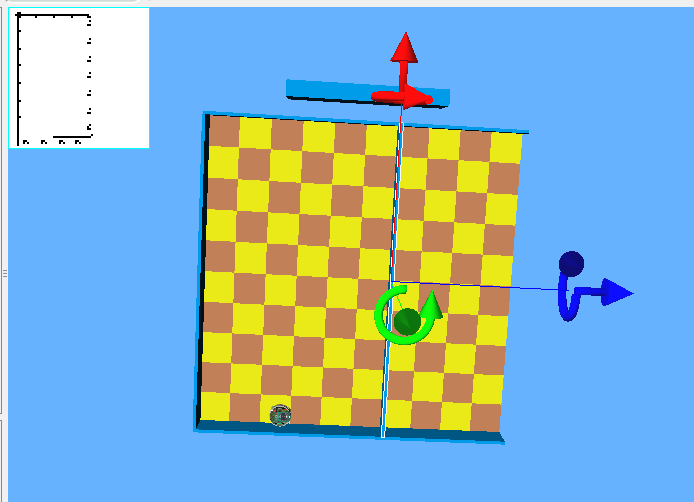
\includegraphics[width = 0.5\textwidth]{../../figures/map_results/save_corner_with_odometry_error.png} 
\caption{Room 2 results}
\label{room2_results}
\end{figure}

Figure \ref{room2_results} shows the result of the second test environment. 
While the map is not finished, the robot was stuck in an eternal loop at the lower wall of the environment.\\
This environment shows once more that the mapping works fine as long as the localisation error has not accumulated it self to much. \\

\begin{figure}[h]
\centering
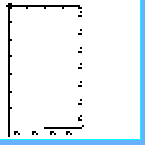
\includegraphics[width = 0.5\textwidth]{../../figures/map_results/minimum_localisation_error.png} 
\caption{Room 2 shows that the localisation error depends on environment size}
\label{room2_error}
\end{figure}

However figure \ref{room2_error} documents also that the increase of the localisation error strongly depends on the size of the environment and there by how far the robot traverses between each wall. \\
The localisation error strongly changes when the robot driver longer distances, even on straight lines. Even if the robot is perfectly calibrated which prevents curves movement caused by different wheel diameters \textbf{FIXME(insert link to where this is discussed in chapter 3)}, the robot will never turn an exact amount of degrees, this is caused by the friction between the wheels and the floor. \\
This however, as already discussed in chapter 3, leads to the robot believing it is somewhere while it actually is somewhere else.  As figure \ref{room2_error} documents this error is reduced if the robot does not need to drive far until it has to turn again.\\
It does so by showing clearly that localisation error, while it still persists, is much smaller than in an empty environment where to robot has to drive further distances until turning. An example of this can be seen in\textbf{ FIXME(add link to localisation error as discussed in chapter 3).} \\[3ex] 

\begin{figure}[h]
\centering
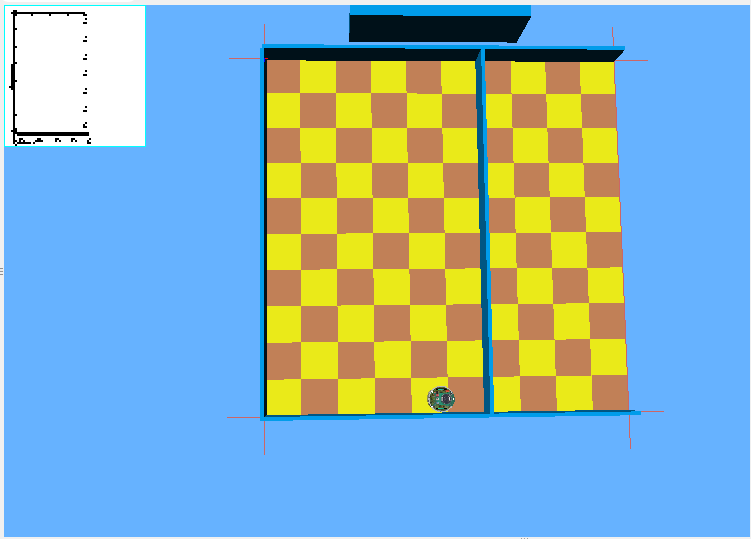
\includegraphics[width = 0.5\textwidth]{../../figures/map_results/save_corner_with_odometry_error_later.png} 
\caption{Room 2 results at a later point}
\label{room2_results_later}
\end{figure}

However the localisation error is not the only problem. As can be seen in figure \ref{room2_error} also in this case the robot reaches an uncharted reference point before passing by an existing reference point to reset its localisation values. This leads to the same problem encountered in section \ref{room1_obstacles}. \\
However the robot in this case is stuck within an eternal loop, where it resets to the right coordinates at the lower-left hand corner and drives to the right-hand side of the map where it gets reset to the wrong localisation values again. \\
The problem of this happening is a bug inside the code combined with odometry errors. The odometry error causes the robot to not directly drive close to the wall but rather stay a bit away from it. And the bug causes the robot to not change it overall direction whenever it reaches one of the corners but rather to stay in the U-Turn movement pattern.

\subsubsection{Conclusion of this test environment}
This test environment did not really showcase any other problems with code then the ones already covered in section \ref{room1}. It did however show case an until now unknown bug which would need to be patched out, if more time were available.\\
This test environment however documented, the already existing assumption, that the size of the localisation error depends on how long distances the robot needs to move until turning again. This localisation error in the first place is however caused by inaccurate turning caused by friction in the environment. 

\subsection{Environment with obstacles}
In this subsection the test results an environment which has the same size as \textbf{room 2}, however holds an extra obstacle.\\

\begin{figure}[h]
\centering
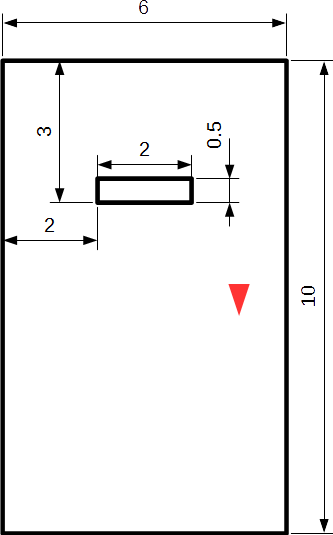
\includegraphics[width = 0.5\textwidth]{../../figures/room2_obstacle.png} 
\caption{Room 2 with obstacles measurements}
\label{room2_obstacles}
\end{figure}

Figure \ref{room2_obstacles_result} shows the result of this test environment. \\
As it can clearly be seen the map of this environment is not finished, the reason for that are bugs in the code and odometry errors.
The robot starts at the marked starting position, red arrow, and proceeds to map the environment as usual. It can clearly be seen where the robot mapped the outline of the obstacle as it passed it. When the robot passed the upper-left reference point this point is saved as usual. \\
The robot then maps the left-hand side wall of the environment, and saves the lower-left hand corner as usual.\\

\begin{figure}[h]
\centering
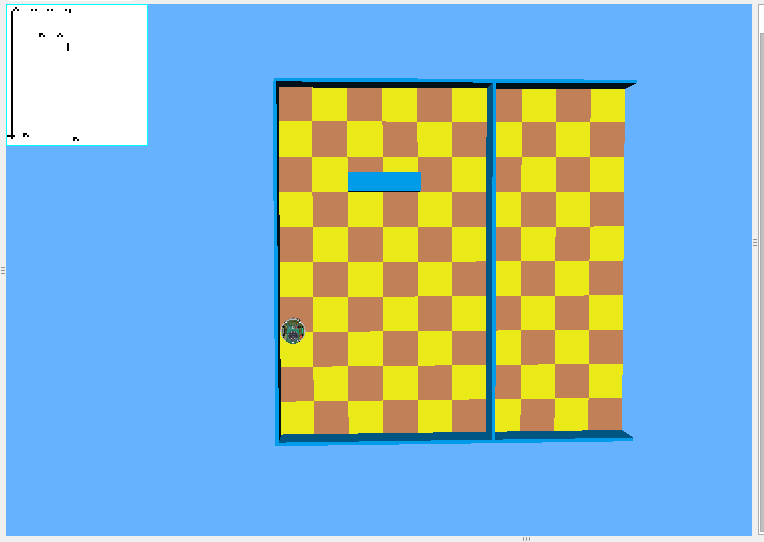
\includegraphics[width = 0.5\textwidth]{../../figures/map_results/room_2_obstacle_result.png} 
\caption{Room 2 with obstacles result}
\label{room2_obstacles_result}
\end{figure}

However here is where the bug in the program causes the robot also save the same corner as the lower-right hand corner and change the direction value of the odometry struct to west wards, while the robot is actually moving north warts.  \\ 
Figure \ref{room2_saving_error} shows the readout generated by the program. It shows how the robot,correctly, moved southwards then saved the corner as corner 1, which is also correct, but then saves the corner also as corner 2 and sets its own direction to west ward, while actually moving to the north.\\[3ex]

This robot then proceeds to move upwards along the left-hand side wall, however the mapping the robot does is outside the map area as it believes to move west ward. The robot drives ~1/4 of the the environment size upwards before the simulator crashes. This crash has happened every single time this environment was tested. 

\begin{figure}[h]
\centering
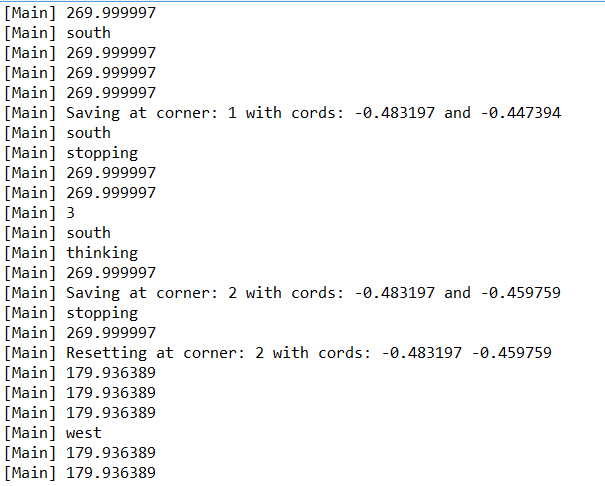
\includegraphics[width = 0.5\textwidth]{../../figures/map_results/room2_saving_error.png} 
\caption{Buggy software causes causes the robot to save wrong values}
\label{room2_saving_error}
\end{figure}

\subsubsection{Conclusion of this test environment}
This test clearly showcases another major bug within the program. Unfortunately not more information can be gather from the test runs as the simulator crashes every time at the same place. 

\section{Room 3}
This section holds the description and results of test of environment \textbf{room 3}. \\
This test environment differs from the previous test environments as it is a more "complex" environment compared to the others. It is more complex as it is completely square, this is done to test the programs performance in a environment like this.\\
This section was also not tested with obstacles inside it. The reason being that the previously gathered data shows that obstacle inside the room disturb the mapping and prevent a complete mapping.
Figure \ref{room3_empty} shows the environment and its measurements. \\

\begin{figure}[h]
\centering
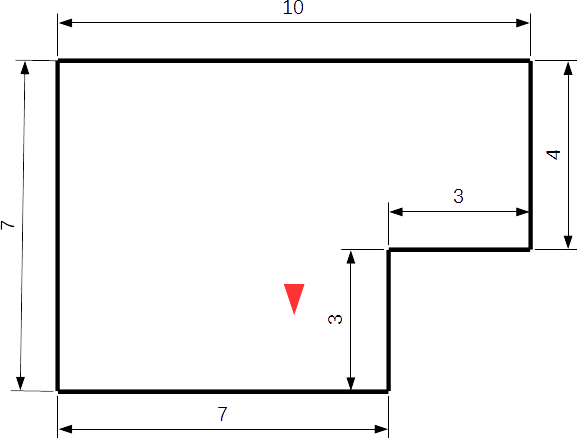
\includegraphics[width = 0.5\textwidth]{../../figures/room3_empty} 
\caption{Measurements of room 3}
\label{room3_empty}
\end{figure}

Figure \ref{room3_result1} shows the map result after the robot traversed a part of the map. It can be seen that the robot mapped the outline of the right-hand wall, however it can be clearly seen that the localisation error accumulated to much which prevents an accurate mapping of the lower wall. \\

\begin{figure}[h]
\centering
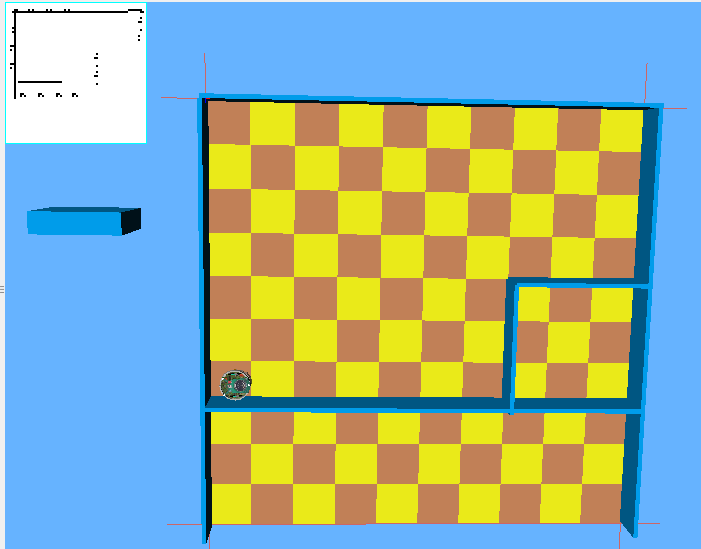
\includegraphics[width = 0.5\textwidth]{../../figures/map_results/room4_result1.png} 
\caption{Result of the third room}
\label{room3_result1}
\end{figure}

It resets the localisation values at the lower left corner, however then proceeds to reset the values to the equivalent of the upper-right corner immediately. The robot then starts to move back and forth along the lower wall, then proceeded to move up the left wall. \\
It resets the localisation values again when the lower-left hand corner is reached for the second time, then moves upwards along the left wall, however the odometry struct now holds the wrong orientation values: the robot believes to move east(to the right).
The robot then proceeded moving along the walls in the normal movement pattern, however with the localisation and orientation values all wrong the mapping was unusable, and the test was ended at this point. 

\subsection{Conclusion of this test environment}
This test environment did not produce a lot of new insight into the final program. While it documented the shortcomings of the reference point algorithm this is not new data, as previous test environments showed the same data. \\
The partly created map with can be seen in figure \ref{room3_result1} indicated that the mapping process of the wall formation at the lower right side of the environment would have been lacking at best. This is based on the moving pattern where the robot moves given distances in the turns, should an wall or obstacle not be "luckily" lay to the side of this path chances are that the robot will not be able to map it, in best cast map the outline. \\

\section{Conclusion}
The test results inside this chapter give clear insight into the weak and strong sides of the program.\\
Unfortunately there are more weak points. During the implementation phase of the project a couple of problems were encountered, problems with odometry, localisation and mapping. While these problems were countered and fixed the solution seamed good inside the implementation environment. This is the main reason why some of the programs shortcomings exist.\\[3ex]

The algorithm which handles the reference points is based on prior knowledge which was gathered during test runs in the implementation phase. It was known prior to design of the algorithm in which direction the robot is moving and from what direction it will approach a corner of the environment. This approach works fine inside the \textbf{room 1} environment but \textbf{room 2} and \textbf{room 3} have shown that this approach failed if the robot should move in a slightly different path than to the one the algorithm was designed under. \\
If the robot reaches a corner but its direction is different from the one specified in the algorithm, it will set or reset its localisation values to different corners than it should. This problem however could be fixed by adding more control statements to the algorithm, rather than simple approach which is implemented at this moment. \\[3ex]

Another weak point of the program is the movement pattern, if obstacles are placed inside the environment their presence can disturb the movement pattern enough to cause severe odometry and localisation errors. It has been observed in the testing phase that an E-Puck has collided with the wall, but rather than to stop it continued driving, however skewed itself along the side of the obstacle changing it path and increasing the localisation error. While this can happen because of the absence of bumper sensors of the E-Puck robot platform and the placement of the distance sensors around the E-Puck's top side, it shows that this robot platform is not the best suited for map building.\\
Another example is the mapping of\textbf{room 3 }which can be seen in figure \ref{room3_result1} and the obstacle mapping of \textbf{room 1} from figure \ref{obstacle_mapping_error}. These 2 figures show the problems with the current movement pattern on walls and obstacles. There is no direct way of fixing the movement pattern in this program. One approach could be to add a wall-following algorithm to whenever a new obstacle is detected, or in case a completely different approach, some of them were discussed in Chapter 1 and 2. \\[3ex]

The biggest problem however is the localisation approach. \\
The localisation error accumulated over time and needs to be reset at some points during the program run in order to prevent large mapping errors which can be seen in all test cases. One of the aims with this project was to be able to localise the robot without the need of GPS or Compass data or long range scanners which can keep track of global reference points at all times. However odometry calculations , which is what was used to locate the robot in this project, have limitations. In a non-perfect environment(an environment without friction or sensor noise) odometry calculations are always going to be an estimate at best, this was the biggest challenge of this project from the very beginning. Without functioning odometry algorithms it was not able to turn the robot an accurate amount of degrees or move it a given distance, even though these algorithms were successfully implemented they are not 100\% accurate, because of friction and sensor noise. \\[3ex]

Without the ability to calculate how much the robot has moved or turned it was impossible to locate the robot accurately. 
The localisation and movement algorithms in them self function perfectly, however since odometry calculations are really just estimated odometry and localisation errors accumulated over time. Functions were created to tackle these problems, algorithms which check the robots heading and ensure it is only ever deviating with a maximum threshold from their path, and to set reference points at points the robot is able to locate, the corners. However the algorithm which controls the heading is only ever accurate as long as the calculated orientation values are right, extreme odometry errors or collisions with walls/obstacles can lead to errors, as the robot posses no possibility to check the actual position and heading in the simulator\footnote{While it is possible to include API functions which return accurate localisation and rotation informations on the virtual robot such functions were never used as they would break the challenges and key points of this project.}.\\
Even considering a case where the heading control algorithms work completely fine(in most cases they do) the localisation error still increases over time. The algorithm designed to set reference points and reset the robots localisation values helped with this problem, however the short comings of this algorithm has already been discussed. \\[3ex]

The overall conclusion drawn on the localisation problem is that is possible to calculate a robot positions, to an extend. However the error will always become to big, and reference points set by the robot it self are unreliable.  While it is completely possible to use odometry calculations to tackle the localisation problem it is necessary to use predefined reference points or GPS and compass data. In order to use predefined reference points very strong and accurate sensors are required, which are not found for each robot platform, as well as the structure of the environment. GPS and compass data would make the localisation as accurate as possible. Of course GPS sensors have also a limited accuracy but the result will certainly be better than without GPS data. An possible approach could also be to combine GPS and odometry calculations to decrease the localisation error as much as possible. \\[3ex]

To summarize the overall conclusion of this project it can be said that, while the program does not perform well or manage to generated accurate maps(unless it is \textbf{room 1}, it has certainly been a learning experience. It has shown the limitations of solely odometry based systems and have given some insight in how to minimize odometry errors, even though it is impossible to remove them completely. \\
The program in itself has strong problems, the movement pattern is far from optimal, but ideas and insight on this was gathered as well. The test have shown the limitations of the implemented algorithms as soon as it was tested on more complex environment, but also provided informations on these shortcomings and ideas on these could be fixed in the future. 




